\newcommand\version{v1}
\problemname{Friends}
$N$ friends are playing a game. Each friend stands at some integer coordinates between $0$ and $L - 1$, at most one friend on each
coordinate. At each step of the game, one friend jumps to a new (non-occupied) location.

After completion of the jump, the \emph{score} of the game is the number of friends who have a friend either
immediately to the right or immediately to the left. At various times during the game,
the friends wonder what their current score is.

\section*{Example}
Assume that we have $N = 3$ friends playing on a strip of length $L = 7$. Initially,
their locations are $1, 3, 4$. The score for this position would be $2$, since 
the friends at position $3$ and $4$ stand beside each other.

The first jump is from position $4$ to $2$, making the new positions $1, 2, 3$. Here, all friends
have someone next to them, so the score is $3$.

The second and final jump is from $3$ to $0$, resulting in the positions $0, 1, 2$. All friends
still have someone next to them, so the score is still $3$.

\begin{figure}[h!]
  \centering
  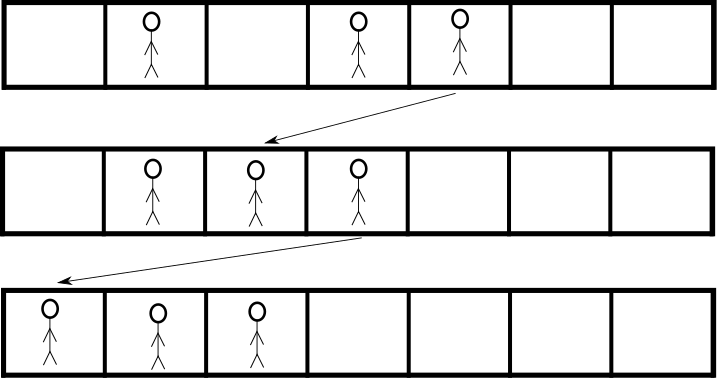
\includegraphics[width=0.8\textwidth]{sample.png}
  \caption{Illustration of the example}
\end{figure}

\section*{Task}
You will get all the jumps in the game, one by one. At some point, the friends will ask what the current score is. Your task is to
implement the functions \texttt{init(N, L, P)}, \texttt{jump(A, B)}, and \texttt{score()}:
\begin{itemize}
  \item \texttt{init(N, L, P)} - this function will be called exactly once by the judge, at the start of the game.
  \begin{itemize}
    \item \texttt{N}: the number of friends playing.
    \item \texttt{L}: the number of locations the game is being played on.
    \item \texttt{P}: an array with $N$ elements. \texttt{P[i]} ($0 \le i < N$) contains the original position of the $i$:th friend.
    \item The function has no return value.
  \end{itemize}

  \item \texttt{jump(A, B)} - this function will be called once for every jump, in the order they are made.
  \begin{itemize}
    \item \texttt{A}: the position a friend is jumping from ($0 \le A < L$). This position will always contain a friend at the time of the jump.
    \item \texttt{B}: the position a friend is jumping to ($0 \le B < L$). This position will never contain a friend at the time of the jump.
    \item The function has no return value.
  \end{itemize}

  \item \texttt{score()} - this function will be called when the friends wish to know their current scure.
  \begin{itemize}
    \item The function should return the current score in the game.
  \end{itemize}

\end{itemize}

\section*{Subtasks}
The problem consists of a number of subtasks. Each subtask gives some amount of points, and to pass
the subtask you must pass all the test cases in the subtask.

\begin{tabular}{|l|l|l|}
  \hline
  \textbf{Subtask} & \textbf{Points} & \textbf{Limits} \\ \hline
  1 & 9 & $1 \le N \le 1\,000$, at most $1\,000$ calls to \texttt{jump} and \texttt{score} will be made. \\ \hline
  2 & 17 & $1 \le N \le 100\,000$, no calls to \texttt{jump} and at most $1$ call to \texttt{score} will be made. \\ \hline
  3 & 14 & $1 \le N \le 10^9$, no calls to \texttt{jump} and at most $1$ call to \texttt{score} will be made. \\ \hline
  4 & 38 & $1 \le N \le 100\,000$, at most $100\,000$ calls to \texttt{jump} and \texttt{score} will be made. \\ \hline
  5 & 22 & $1 \le N \le 10^9$, at most $100\,000$ calls to \texttt{jump} and \texttt{score} will be made. \\ \hline
\end{tabular}

\section*{Input format}
The sample judge reads input in the following format:

\begin{itemize}
  \item line $1$: \texttt{N L Q}
  \item line $2$: \texttt{P[0] P[1] .. P[N - 1]}
  \item lines $2$ to $2 + Q - 1$: each line represents either a jump or a score question.
    If the line is \texttt{0 A B}, a jump from $A$ to $B$ is to be made, and if the line is \texttt{1} a scoring question is to be made.
\end{itemize}

\section*{Output format}
For each scoring question, the judge writes a line with the return value of \texttt{score()}.
